% Visible-stroke transcription; D? and the retraced side connections remain unresolved.
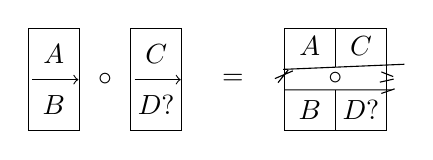
\begin{tikzpicture}[x=.65cm,y=.65cm]
\draw (0,0) rectangle (1,2); \draw[->] (.08,1)--(.98,1);
\node at (.5,1.5) {$A$};\node at (.5,.5) {$B$};
\node at (1.5,1) {$\circ$};
\draw (2,0) rectangle (3,2);\draw[->] (2.08,1)--(2.98,1);
\node at (2.5,1.5) {$C$};\node at (2.5,.5) {$D?$};
\node at (4,1) {$=$};
\draw (5,0)--(7,0)--(7,2)--(5,2)--cycle;
\draw (5,.8)--(7.1,.8) (4.98,1.2)--(7.35,1.3);
\draw (6,0)--(6,.8) (6,1.25)--(6,2);
\node at (5.5,1.65) {$A$};\node at (6.5,1.65) {$C$};
\node at (5.5,.4) {$B$};\node at (6.5,.4) {$D?$};
\node at (6,1.02) {$\circ$};
% Plain crossing strokes preserve uncertainty and do not declare arrows.
\draw (4.82,1.02)--(5.17,1.17) (4.88,.94)--(5.08,1.19);
\draw (6.9,1.15)--(7.13,1.06) (6.87,.95)--(7.14,1.01)
 (6.9,.73)--(7.16,.82);
\end{tikzpicture}
